\chapter{Gases of Moving Atoms}
In experiments, the atomic motion including collisions is another important factor that might impact the optical response of the gas. We have to face the possibility that the influence from the kinematics of atoms could be so remarkable that some cooperative effects may be more or less swept under the rug. Therefore, it is worthwhile to extend our simulations to moving atoms. 

Subsequent to the simulations on inhomoneneous broadened stationary atomic samples, we develop a program to deal with the atomic motions and the time evolution of dipole moments. 

Similarly, inhomogeneous broadening included in the simulations of moving atoms for it is a natural consequence of a thermal velocity distribution. Just as in the stationary-atom model, given a certain spacial distribution, we would be able to solve a closed set of linear equations to obtain the dipole moment of each atom.  However, in the moving-atom model, we integrate the equation of motion of each atom's dipole moment until the gas eventually reaches an equilibrium. During that time, atoms undergo free flight as well as elastic collisions with the container walls and other atoms. Accordingly, we find that some kinematic factors such as the frequency of collisions, may kick in to affect the simulation outcomes.

As expected, some results of stationary-atom simulations are inherited by moving-atom simulations, such as the dependence of collective Lamb shift on the sample thickness. Beyond that, some new features that do not exist in stationary-atom model could emerge. For instance, a typical Dicke narrowed lineshape~\cite{PhysRev.89.472} is observed. This is not surprising. After all, in reality, atoms are not stationary and Dick narrowing has been indeed observed.

However, contrary to what one might predict, as the gas density rises, the width of the Dick narrowed central peak is increasing. This is quite unlike what would happen in a hypothetical gas of independent atoms, wherein the higher density would reduce the linewidth. We attribute this broadening to the strong dipole-dipole interactions between the atoms, or from an overall perspective, the cooperative response of the gas to light. 

The following discussion is constructed similarly as last chapter of stationary atoms. We will start from the analysis of one single moving atom, extend to many independent atoms and finally focus on atoms with dipole-dipole interactions. Of course, all the calculations and simulations are done in a circular slab.

\section{Calculation of A One-atom Gas}
In our model of discrete dipolar radiators, Eq.~\eq{CORE} can be specified so that it describes the time evolution of each atom's dipole moment. For the $n$th atom located at $\mathbf{r}_n$, we have
\bea
\dot{\mathbf{d}}(\mathbf{r}_n)&=&(i\Delta-\gamma)\mathbf{d}(\mathbf{r}_n)+i\zeta\mathbf{\mathcal{E}}_0(\mathbf{r}_n)+i\zeta\sum_{m\neq n}\mathsf{G}(\mathbf{r}_n-\mathbf{r}_m)\mathbf{d}(\mathbf{r}_m).
\label{DIPOLEEQ}
\eea
As before, $\Delta=\omega-\omega_0$ is the detuning from the atomic resonance $\omega_0$, $\gamma$ is the HWHM line width of the transition, $\zeta=\mathcal{D}^2/\hbar$ and $\mathcal{D}$ is the dipole matrix element and $\mathbf{\mathcal{E}}_0$ is the electric field of the driving light if the matter were absent. $\mathsf{G}(\mathbf{r}_n-\mathbf{r}_m)$ is the dipole field propagator from the atom at $\mathbf{r}_m$ to the atom at $\mathbf{r}_n$.

It is worth reminding that atomic motion is taken into account in our model, hence $\mathbf{r}_n$ is actually a function of time and coordinates change with time as the atoms move.

The first term on the right hand side of Eq.~\eq{DIPOLEEQ} comes from the damped free evolution of the atomic polarization. The second and the third terms, respectively, correspond to the polarization induced by the incident light and the scattered light from all the other atoms. Apparently, if the left hand side of Eq.~\eq{DIPOLEEQ} equals zero, this equation would be reduced to a steady state as given by Eq.~\eq{STEADY}.

All the calculations and simulations we present below are all done with these universal configurations:


First, the gas sample is inside a circular disk with thickness $h$ and radius $R$. For convenience, the disk is placed so that its axis is used as the $z$ axis, and the body center is the coordinate origin.

Second, the incident light is represented by $\mathcal{E}_0(\mathbf{r})=E_0\,\hat{\mathbf{e}}\,e^{i\mathbf{k}\cdot\mathbf{r}}$. It is circularly polarized and the propagating in the $+z$ direction.
\bea
\hat{\mathbf{e}}=\{\frac{1}{\sqrt{2}},\frac{i}{\sqrt{2}},0\}, \, \mathbf{k}=\{0,0,1\}.
\eea

Third, the absorption spectrum is investigated by calculating the optical thickness $D$ of the sample, as defined in Ref~cite{0953-4075-44-19-195006}. Details will be given later.

Finally, the units we use are the same as for stationary atoms:
\bea
k=c=\hbar=\frac{1}{4\pi\epsilon_0}=1,
\eea 
and linewidth of the transition $\gamma$ and dipole matrix element $\mathcal{D}$ are still related by 
\bea
\mathcal{D}=\sqrt{\frac{3\gamma}{2}}.
\eea

\subsection{Dipole Evolution of the Atom}
If the gas consists of only one atom, Eq.~\eq{DIPOLEEQ} can be reduced to a nonhomogeneous first-order ODE:
\bea
\dot{\mathbf{d}}(t)+(1-i\delta)\mathbf{d}(t)=i\frac{3}{2}\mathcal{E}_0(t)=i\frac{3}{2}E_0\,\hat{\mathbf{e}}\,e^{i\mathbf{k}\cdot\mathbf{r}(t)},
\label{SINGLEEQ}
\eea
where $\delta=\Delta/\gamma$ and the dependence on position is expressed in the form of a dependence on time. 

For $\mathbf{k}=\{0,0,1\}$, we readily have $\mathbf{k}\cdot\mathbf{r}(t)=z(t)=z_0+v_zt$. Thus, the radial components of the initial position and the velocity have no impact on the evolution. So we need not concern with the collision between the atom and the lateral surface of the disk at all. As we will see later, even $z_0$ does not matter either. Therefore, we would not hesitate to endow the atom with $\mathbf{r}_0=\{0,0,-h/2\}$ and $\mathbf{v}_0=\{0,0,v\}$ to carry out our calculations. This atom is sufficient to represent all the atoms that have the same axial speed. Here, $v$ must be positive because the atom is initially at $z=-h/2$, the atom has to be moving in the $+z$ direction.

With the given assumptions, we have $\mathbf{d}_0=-\frac{3}{2(i+\delta)}E_0e^{-i\frac{h}{2}}\hat{\mathbf{e}}$ as the initial dipole moment for the evolution. As a matter of fact, the equilibrium state that the system would reach after a large number of collisions is independent of the initial state. Anyway, given $\bf{d}_0$, the solution to Eq.~\eq{SINGLEEQ} is
\bea
d(t)&=&-\frac{3E_0}{2(i+\delta-v)}e^{i(-h/2+vt)}\left[1-e^{-t+i(\delta-v)t}\right]+e^{-t+i\delta t}d_0
\label{SINGLESOL}
\eea
Note that we do not use the bold font any more because the dipole moment always has the same polarization as the incoming electric field, so $\hat{\mathbf{e}}$ can be eliminated in the equation and every thing now is scalar.

Obviously, the first term in Eq.~\eq{SINGLESOL} depends on the velocity and the instantaneous electric field at the ever-changing position of the atom. The second term is the damping of the initial state. In free space, as time tends to infinity, the dipole moment would asymptotically approach
\bea
d(t\to\infty)=\alpha(v)E_0e^{i(-h/2+vt)},
\eea
where $\alpha(v)\equiv-\frac{3}{2(i+\delta-v)}$ is the Doppler-shifted polarizability of the atom with speed $v$.

If the atom is restricted in a circular disk region so it experiences elastic collisions at $z=\pm h/2$, the direction of the velocity reverses after each collision. The time interval between any two successive collisions  is $h/v$. When the first collision happens at $z=h/2$, the dipole becomes
\bea
d_1\equiv d(t=\frac{h}{v})&=&\alpha(v)E_0 e^{ih/2}\left[1-e^{-\frac{h}{v}+i(\delta-v)\frac{h}{v}}\right]+e^{-\frac{h}{v}+i\delta \frac{h}{v}}d_0.
\eea

$d_1$ would in turn serve as the initial state to obtain the dipole at the second collision $d_2$. Note that this time $v$ is replaced by $-v$ for the atom would bounce back after the first collision:
\bea
d_2&=&\alpha(-v)E_0e^{-ih/2}\left[1-e^{-\frac{h}{v}+i(\delta+v)\frac{h}{v}}\right]+e^{-\frac{h}{v}+i\delta \frac{h}{v}}d_1\nonumber\\
&=&\alpha(-v)E_0e^{-ih/2}\left[1-e^{-\frac{h}{v}+i(\delta+v)\frac{h}{v}}\right]+\alpha(v)E_0e^{ih/2}\left[1-e^{-\frac{h}{v}+i(\delta-v)\frac{h}{v}}\right]e^{-\frac{h}{v}+i\delta \frac{h}{v}}\nonumber\\
&&+(e^{-\frac{h}{v}+i\delta \frac{h}{v}})^2d_0\nonumber\\
&=&d_+q+d_-+q^2d_0.
\eea

Here we have defined
\bea
d_+&=&\alpha(v)E_0e^{ih/2}\left[1-e^{-\frac{h}{v}+i(\delta-v)\frac{h}{v}}\right],\nonumber\\
d_-&=&\alpha(-v)E_0e^{-ih/2}\left[1-e^{-\frac{h}{v}+i(\delta+v)\frac{h}{v}}\right], \nonumber\\
q&=&e^{-\frac{h}{v}+i\delta \frac{h}{v}}
\eea
for an even more compact notion.

Now we can inductively write out the dipole moment at the $n$th collision as 

\begin{subequations}
\begin{numcases}{d_n=}
d_+\sum_{k=0}^{\frac{n-1}{2}}q^{2k}+d_-\sum_{k=0}^{\frac{n-3}{2}}q^{2k+1}+q^nd_0, &($n$ is odd and $n\geq 3$) \\
 \nonumber\\
d_+ \sum_{k=0}^{\frac{n-2}{2}}q^{2k+1}+d_- \sum_{k=0}^{\frac{n-2}{2}}q^{2k}+q^nd_0. &($n$ is even and $n\geq 2$)
\end{numcases}
\end{subequations}
Since $\left|q\right|<1$, the summations converge as $n\to\infty$ so that:
\begin{subequations}
\begin{numcases}{d_{n\to\infty}=}
\frac{d_++qd_-}{1-q^2}, \, & \textrm{(if $n$ is odd)}\label{FINAL1}\\
\nonumber\\
\frac{qd_++d_-}{1-q^2}. \, & \textrm{(if $n$ is even)}\label{FINAL2}
\end{numcases}
\end{subequations}

If we wait long enough, the time evolution of the dipole moment would eventually develop into an oscillation between the states of~\eq{FINAL1} and~\eq{FINAL2}, when the system reaches the equilibrium. Namely, at equilibrium, the dipole moment is equal to ~\eq{FINAL1} when the atom arrives at the base at $z=h/2$ and equal to ~\eq{FINAL2} when it is at $z=-h/2$.

Between the two bases, the dipole moment still evolves according to Eq.~\eq{SINGLESOL}. The oscillation of the dipole moment is synchronized with the kinematic oscillation. The period of both oscillations equals the duration of a round trip between the two bases, which is $2h/v$.

Consider the dipole moment in just one period, if we zero the timer when the atom is at $z=-h/2$, in the first half period the dipole moment is given by
\bea
d_{F}(t)&=&\alpha(v)E_0e^{ih/2}\left[1-e^{-t+i(\delta-v)t}\right]+q(qd_++d_-)\frac{1}{1-q^2}.
\label{FORWARD}
\eea

We zero the timer again when the atom reaches $z=h/2$, after that, during the return trip, the dipole is
\bea
d_{B}(t)&=&\alpha(-v)E_0e^{-ih/2}\left[1-e^{-t+i(\delta+v)t}\right]+q(d_++qd_-)\frac{1}{1-q^2}.
\label{BACKWARD}
\eea

Combining Eq.~\eq{FORWARD} and Eq.~\eq{BACKWARD}, we are able to write out the dipole moment at any time within one period:
\begin{numcases}{d(t)=}
d_F(t), & (for $0\leq t\leq  h/v$)\nonumber\\
d_B(t-h/v). & (for $h/v \leq t \leq 2h/v)$
\label{BACKFORTH}
\end{numcases}

\subsection{The Optical Thickness}
Now let's investigate the absorption spectrum by calculating the optical thickness $D=\ln\left|\tau\right|^{-2}$, as defined in Ref.~\cite{0953-4075-44-19-195006}.  

First of all, Eq.~\eq{BACKFORTH} is actually an explicit function of $h$, $v$, $\delta$ and $t$. So we write it as $d(h,v,\delta,t)$.

For a single atom as above, the transmission coefficient
\bea
\tau_1=1+\frac{2ie^{-iz(t)}d(h,v,\delta,t)}{R^2E_0},
\eea
where $z(t)$ is the position of the atom at time $t$. 

The optical thickness $D_1$ is
\bea
D_1(h,v,\delta,t)&=&\ln\left|\tau_1\right|^{-2}=-\ln\left|\tau_1\right|^2=-\ln(\tau_1\tau_1^*)\nonumber\\
&=&-\ln\Bigg\{1+2\,\mathfrak{R}\left[\frac{2ie^{-iz(t)}}{R^2}\frac{d(h,v,\delta,t)}{E_0}\right]\nonumber\\
&&+\left|\frac{2ie^{-iz(t)}}{R^2}\frac{d(h,v,\delta,t)}{E_0}\right|^2\Bigg\}.
\eea

For $R\gg1$, we have the approximation such that
\bea
D_1(h,\delta,v,t)&\approx&-\ln\left(1+2\,\mathfrak{R}\left[\frac{2ie^{-iz(t)}}{R^2}\frac{d(h,v,\delta,t)}{E_0}\right]\right)\nonumber\\
&\approx&-\frac{4}{R^2E_0}\mathfrak{R}\left[ie^{-iz(t)}d(h,v,\delta,t)\right].
\label{APPROX}
\eea

As we discussed in Sec. II, $z(t)$ and $d(h,v,\delta,t)$ are oscillating in phase, so the time average of the optical thickness can be calculated by integrating the whole term in the square brackets over a round trip of the atom and dividing the result by $2h/v$, as below.
 \bea
\bar{D}_1(h,v,\delta)&=&-\frac{4}{R^2E_0}\mathfrak{R}\left[\frac{v}{2h}\int_0^{\frac{2h}{v}} ie^{-iz(t)} d(h,v,\delta,t)dt\right]\nonumber\\
&=&\frac{4}{R^2}\mathfrak{R}\Bigg\{\frac{3v^3\left[coth(\frac{h-ih\delta}{v})-\cos(h)csch(\frac{h-ih\delta}{v})\right]}{h(i+\delta-v)^2(i+\delta+v)^2}\nonumber\\
&&-\frac{3(1-i\delta)}{2(i+\delta-v)(i+\delta+v)}\Bigg\}.
\label{THEORYD}
\eea

As a final step, we hypothesize an ensemble consisting of an infinite number of one-atom gas samples, over which the atom's axial velocity obeys a Gaussian distribution and the rms axial velocity (i.e. the standard deviation) equal $u$. Then a formal absorption spectrum is given by:
\bea
D_1(h,u,\delta)=\int_{-\infty}^{\infty}\bar{D}_1(h,v,\delta)\frac{e^{-\frac{v^2}{2u^2}}}{\sqrt{2\pi}\,u}dv.
\label{ONEATOMSPECTRUM}
\eea

According to Eq.~\eq{ONEATOMSPECTRUM}, given certain $h$ and $u$ values, we numerically calculate and plot $D_1$ versus $\delta$ in  Fig.~\eq{SINGLESPECTRUM}. The lines are calculation results and the scatters stand for the simulation outcomes.
\begin{figure}[h!]
\begin{center}
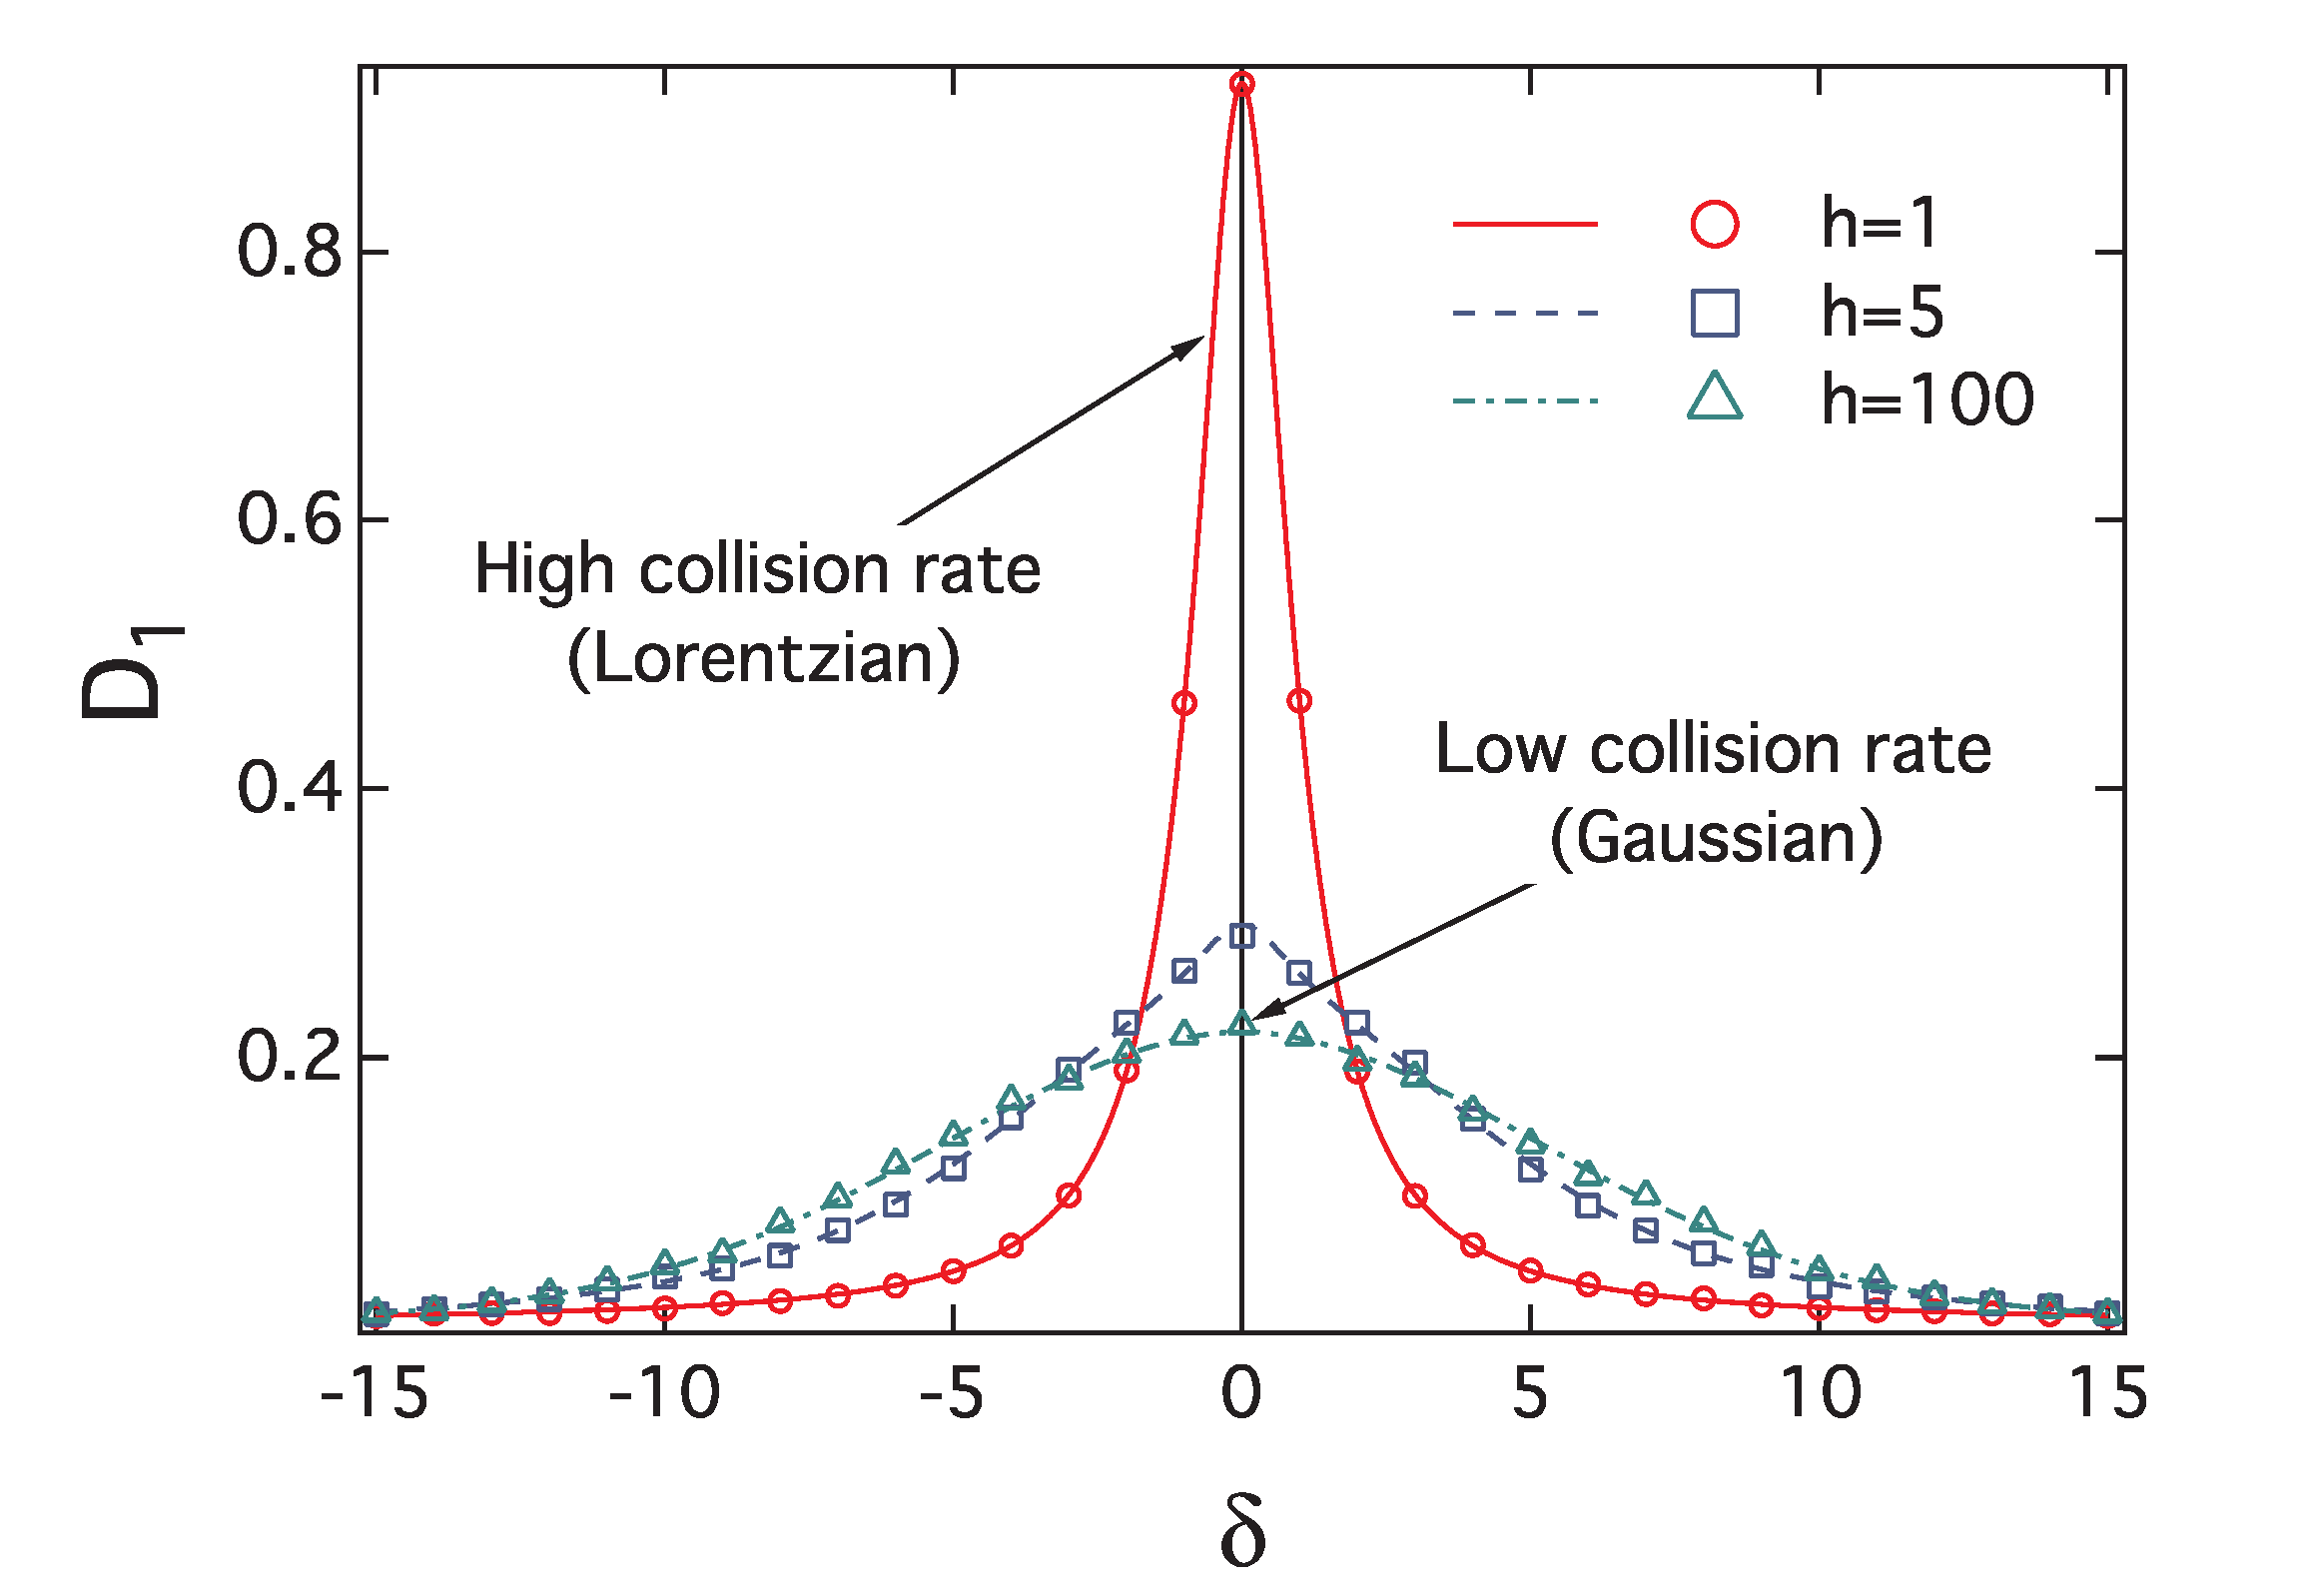
\includegraphics[width=\textwidth]{single_atom.pdf}
\end{center}
\caption{Optical depth $D_1$ versus detuning $\delta$ of a single-atom ensemble with thickness $h=100, 5$ and $1$. The rms axial speed of the atom is $v=5$ for all. Gaussian and Lorentzian profiles are observed when $h=100$ and $h=1$ respectively. When $h=5$, a bulge in the center distorted the curve, making the profile an intermediate state between Gaussian and Lorentzian. Simulations precisely agree with analytical calculations.}
\label{SINGLESPECTRUM}
\end{figure}

The three curves in  Fig.~\eq{SINGLESPECTRUM} also reveal an important phenomenon. As we keep the rms speed of the atom constant and vary the thickness $h$ from extremely big to very small, the spectrum profile undergoes a transition from a broad Gaussian lineshape to a narrow Lorentzian, which is roughly of the natural linewidth.  This narrowing mechanism is consistent with Dicke narrowing. That is to say,  a shorter distance between the two bases, hence a shorter mean free path of the atom, would narrow the spectrum.

\subsection{A Simplified Multiple-Atom Gas}

We can make one more step forward to a simplified model of a gas of $N$ atoms.

In this model, the atom radius is infinitesimal hence there is no atom-atom collision. Moreover, the dipole-dipole interaction between atoms is also neglected. Each atom under these conditions would evolve absolutely independent of others, therefore the dipole moment of each atom at equilibrium is still given by Eq.~\eq{BACKFORTH}. 

If we have $\{v_n\}$ $(n=1,2,3,\cdots,N)$ as the speeds of the $N$ atoms, the total transmission coefficient can be written as:
\bea
\tau_N=1+\sum_{n=1}^{N}\frac{2ie^{-iz_n(t)}d(h,\delta,v_n,t)}{R^2E_0},
\eea
where $z_n(t)$ is the ever-changing position of the $n$th atom. 

Like before, we assume $R\gg 1$, so the approximation in Eq.~\eq{APPROX} is still valid and the total optical thickness of the gas
\bea
D_N(h,\{v_n\}, \delta,t)&\approx&-\frac{4}{R^2E_0}\mathfrak{R}\left[\sum_{n=1}^{N}ie^{-iz_n(t)}d(h,\delta,v_n,t)\right]=\sum_{n=1}^{N}D_1(h,v_n,\delta,t)
\eea

Note that the sum and the time integral in Eq.~\eq{THEORYD} are interchangeable, so the time average is
\bea
\bar{D}_N(h,\{v_n\},\delta)=\sum_{n=1}^{N}\bar{D}_1(h,v_n,\delta)
\eea

Finally, if $\{v_n\}$ obeys Gaussian distribution with rms velocity $u$, the absorption spectrum of the N-atom gas is then
\bea
D_N(h,u,\delta)=ND_1(h,u,\delta)
\eea

We can see that except for a multiplying factor $N$, the spectrum of such a simplified model of gas is essentially identical to the one of a single atom, as in Fig.~\eq{SINGLESPECTRUM}. 
 
This is the end point of the analytical calculations. 

If we want to investigate the influence on the spectrum brought by atom-atom collisions, we have to turn to simulations.

More details about our simulations will be introduced in next section. Here, as a premiere, we present the simulation results for a gas of N atoms with and without atom-atom collisions in Fig.~\eq{COLLISION} (dipole-dipole interaction is still not considered in either case). It is clear that as we adopt a big atom radius so that atom-atom collisions become very frequent, the lineshape is significantly narrowed. 

\begin{figure}[h!]
\begin{center}
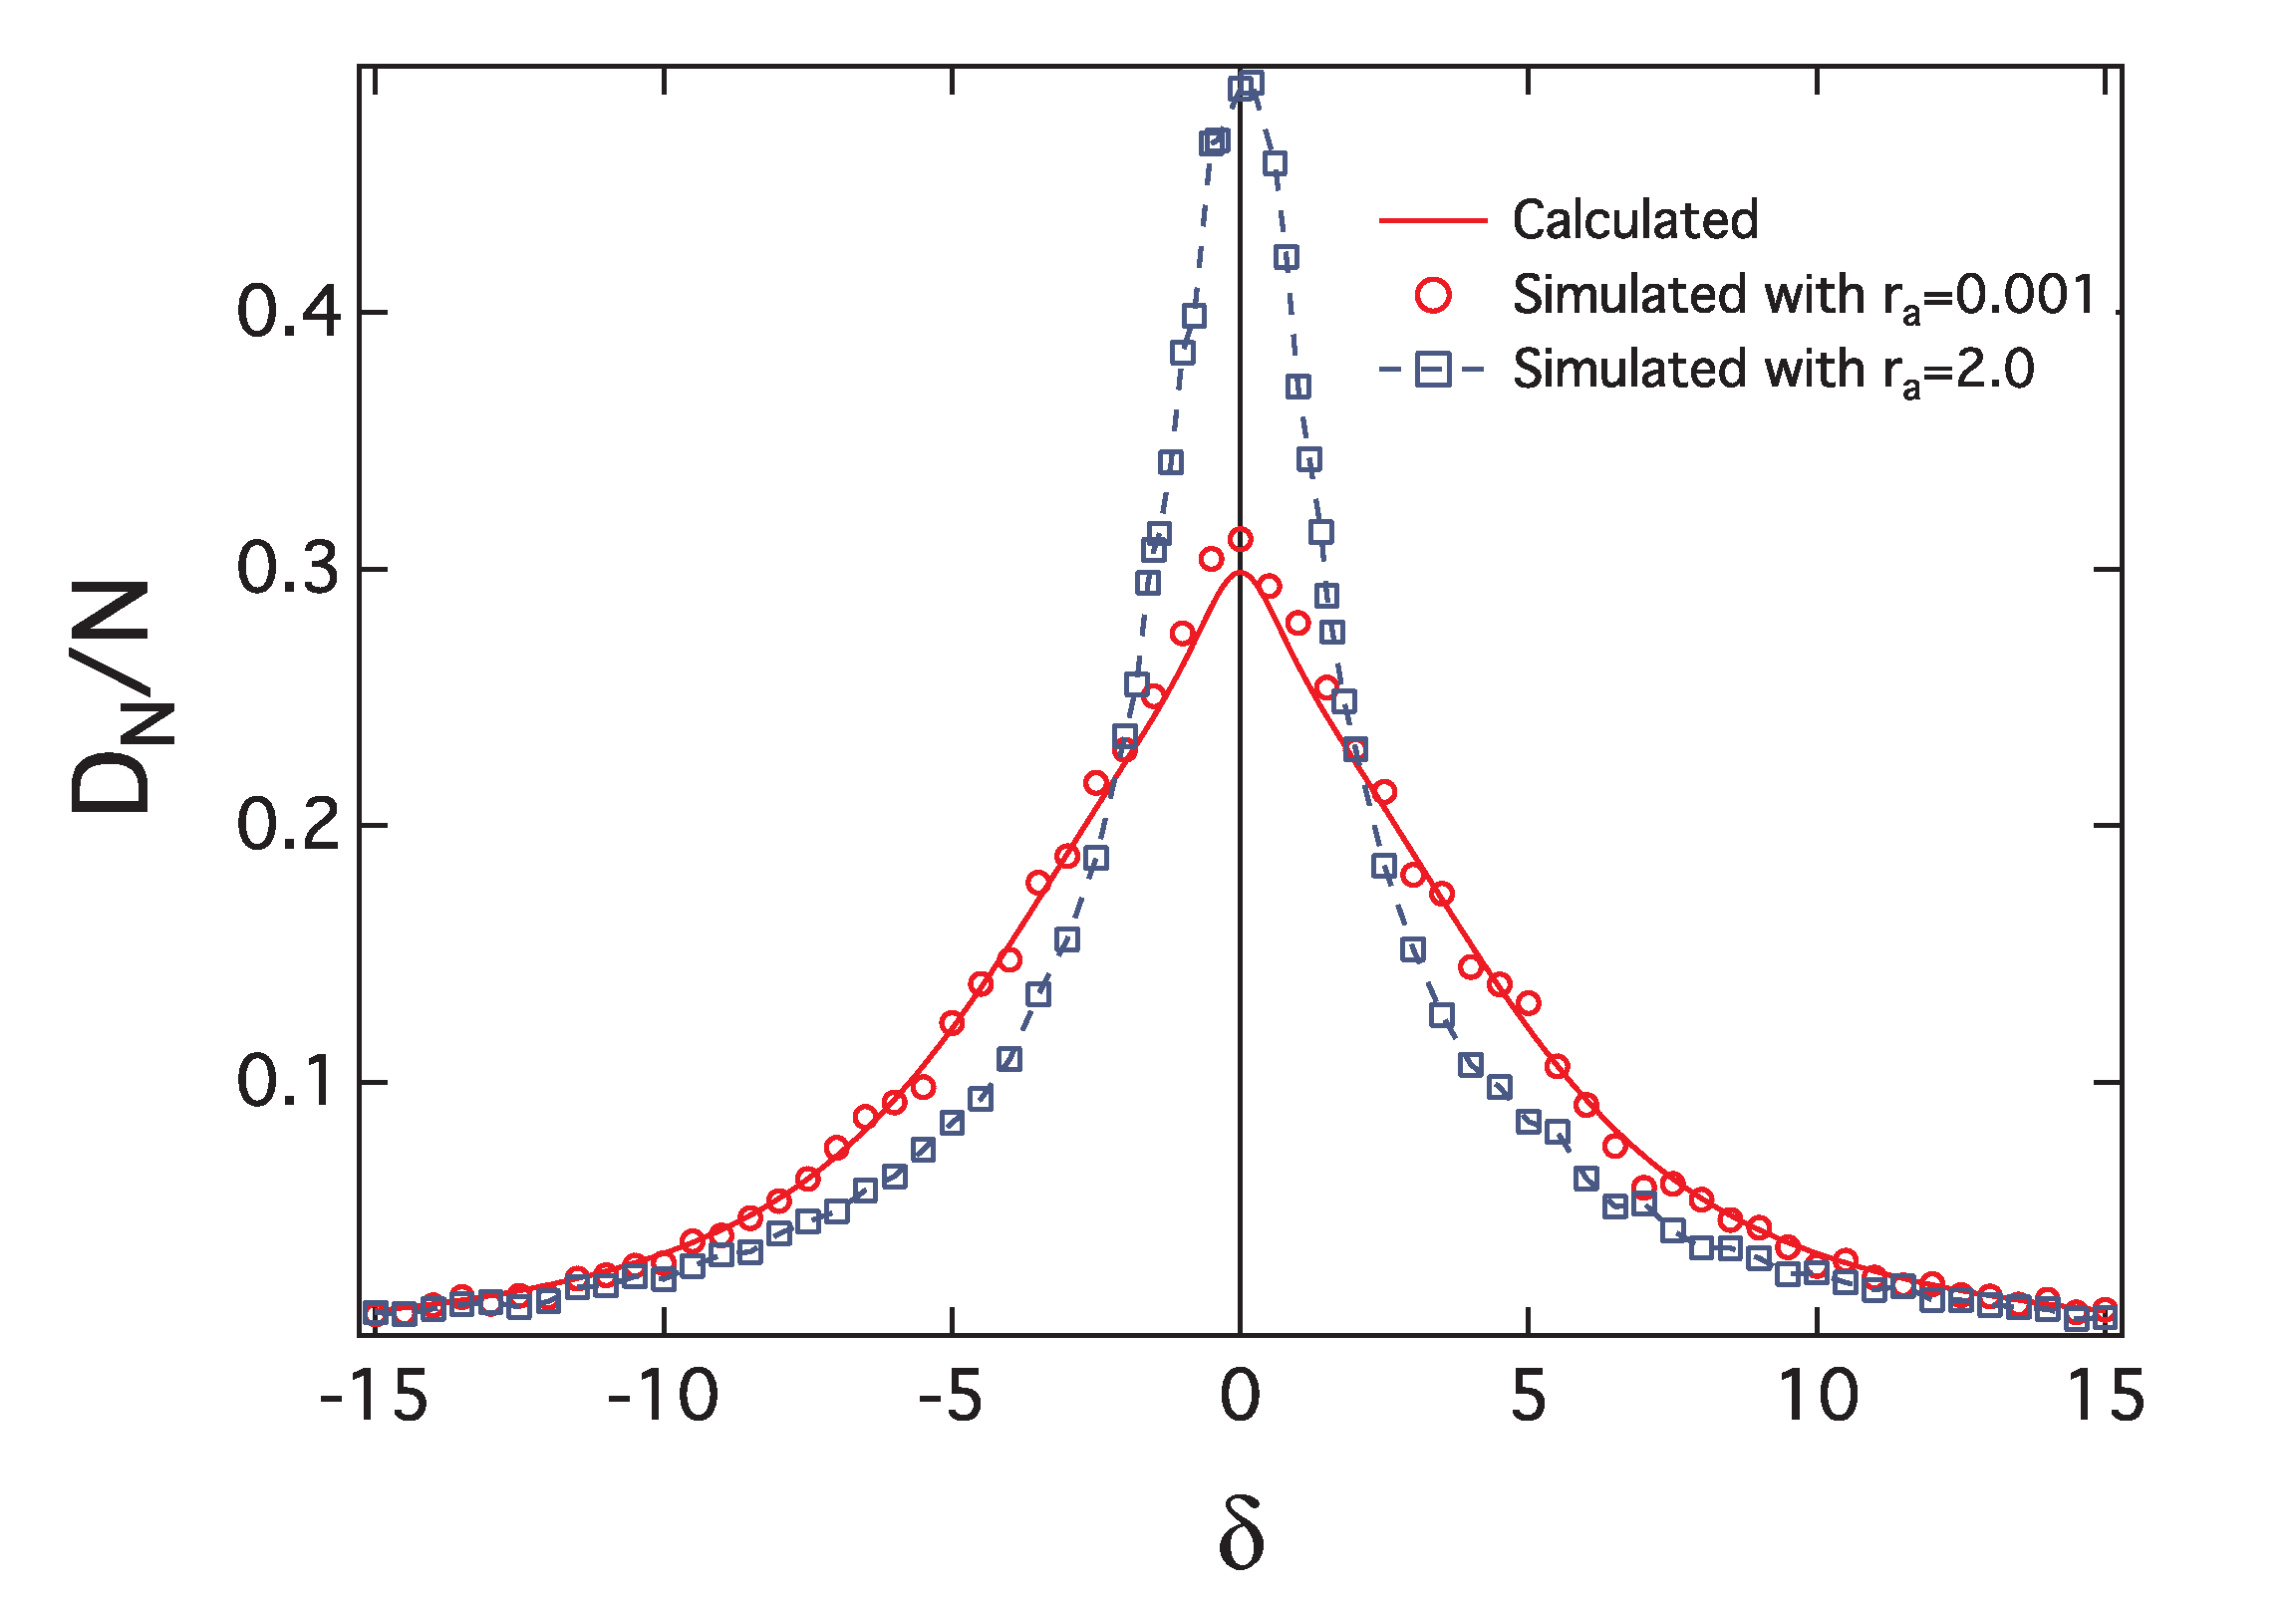
\includegraphics[width=\textwidth]{COLLISION.pdf}
\end{center}
\caption{$D_N/N$ versus $\delta$ with different atom-atom collision ratios. The solid line is calculated by Eq.~\eq{ONEATOMSPECTRUM}, identical to $D_1$ of $h=5$ in Fig.~\eq{SINGLESPECTRUM}. The black crosses correspond to a simulation where atom radius $r_a=0.001$ and the program recorded exactly zero atom-atom collisions. While the red dots correspond to a simulation where $r_s=2.0$ so about half of the collisions are mutual collisions between atoms. In all cases, $N=10$, $u=5$, $R=\sqrt{256/\pi}$ and $h=5+2r_a$. Note that the thickness of the disk has been adjusted to remove any effective shortening of the disk due to the assumption that each atom is a rigid sphere of radius $r_a$.}
\label{COLLISION}
\end{figure}
In summary, if dipole-dipole interactions between atoms are completely absent, either by squeezing the disk in the $z$-direction or by increasing the atom radius, we would end up with a narrower lineshape in the absorption spectrum. Essentially, these two approaches are doing the same thing: reducing the mean free path of the atoms.

\section{Simulations of Multiple-atom Gases}

\subsection{Procedure and Validity of the Simulation Program}

Most of our effort is put into the simulations including dipole-dipole interaction. First of all, some details about our simulations will be introduced. 

\subsubsection{The Initial State of the Evolution}

We assume that, initially, the gas sample is evenly distributed in the circular disk. The atoms obey the Maxwell-Boltzmann velocity distribution and have the same root-mean-squared speed in all three dimensions.

Although the initial states of atoms' dipole moments are irrelevant to the final state as shown in Sec. II, it is still worthwhile to carefully choose the initial states so that the system would relax as soon as possible. This is critical when we deal with a large number of atoms for the time efficiency in computation now becomes a major concern. 

As soon as the incident field is turned on, each atom would be excited by the incident field as well as the dipolar fields from all the other atoms. The time needed to establish the total electric field inside the sample is so short that during which the displacements of the atoms are negligible.  Therefore, we still assume the atoms would stay stationary until the correlations are set up. That means, in our simulations, after the initializations of positions and velocities, the first step is to solve the same hierarchy of equations for the dipole moment of each atom as in a stationary-atom simulation. Just like in the stationary samples, the resonance frequency of each atom has a Doppler shift of $\Delta\omega=kv$. The solutions to these $6N$ linear equations provide the initial states of the dipole evolution described by Eq. ~\eq{DIPOLEEQ}. Essentially, an inhomogeneously broadened static sample in our previous simulations is treated as an initial state in our current simulations. We investigate what would happen when the atoms are moving and colliding.

\subsubsection{Integrating the Evolution Equations and Sampling}

We use adaptive-stepsize Runge-Kutta method to integrate Eq.~\eq{DIPOLEEQ} numerically. The coordinates of the $n$th atom $\mathbf{r}_n$ change with time as the atom moves. Between two successive collisions, the displacement of an atom is simply linear to time. However, this linear dependence would be interrupted by a collision for the velocity always alters its direction in the rigid-sphere model. Consequently, we have to halt the Runge-Kutta integration when a collision happens, update the atom that just collided with the new velocity and then resume the computation.

In the simulations with stationary atoms, we took average over many statistically independent static samples. Now we work on the time average of only one sample instead.  We wait for a time much longer (ten times longer) than the relaxation time of the system, and then begin to take a large number of snapshots of the system's state at times. The time interval between successive snapshots is also longer than the relaxation time to ensure the independence of the samples. Each snapshot works as a sample in our analysis. 


\subsubsection{Collective Lamb Shift: Replicating the Result from Stationary-Atom Simulations}
 
In the simulations of stationary atoms, collective Lamb shifts are observed in dense gases when inhomogeneous broadening is added. For moving atoms,  the CLS is retained as time goes on. This is natural since the model of moving atoms is closer to a real gas.

\begin{figure}[h!]
\begin{center}
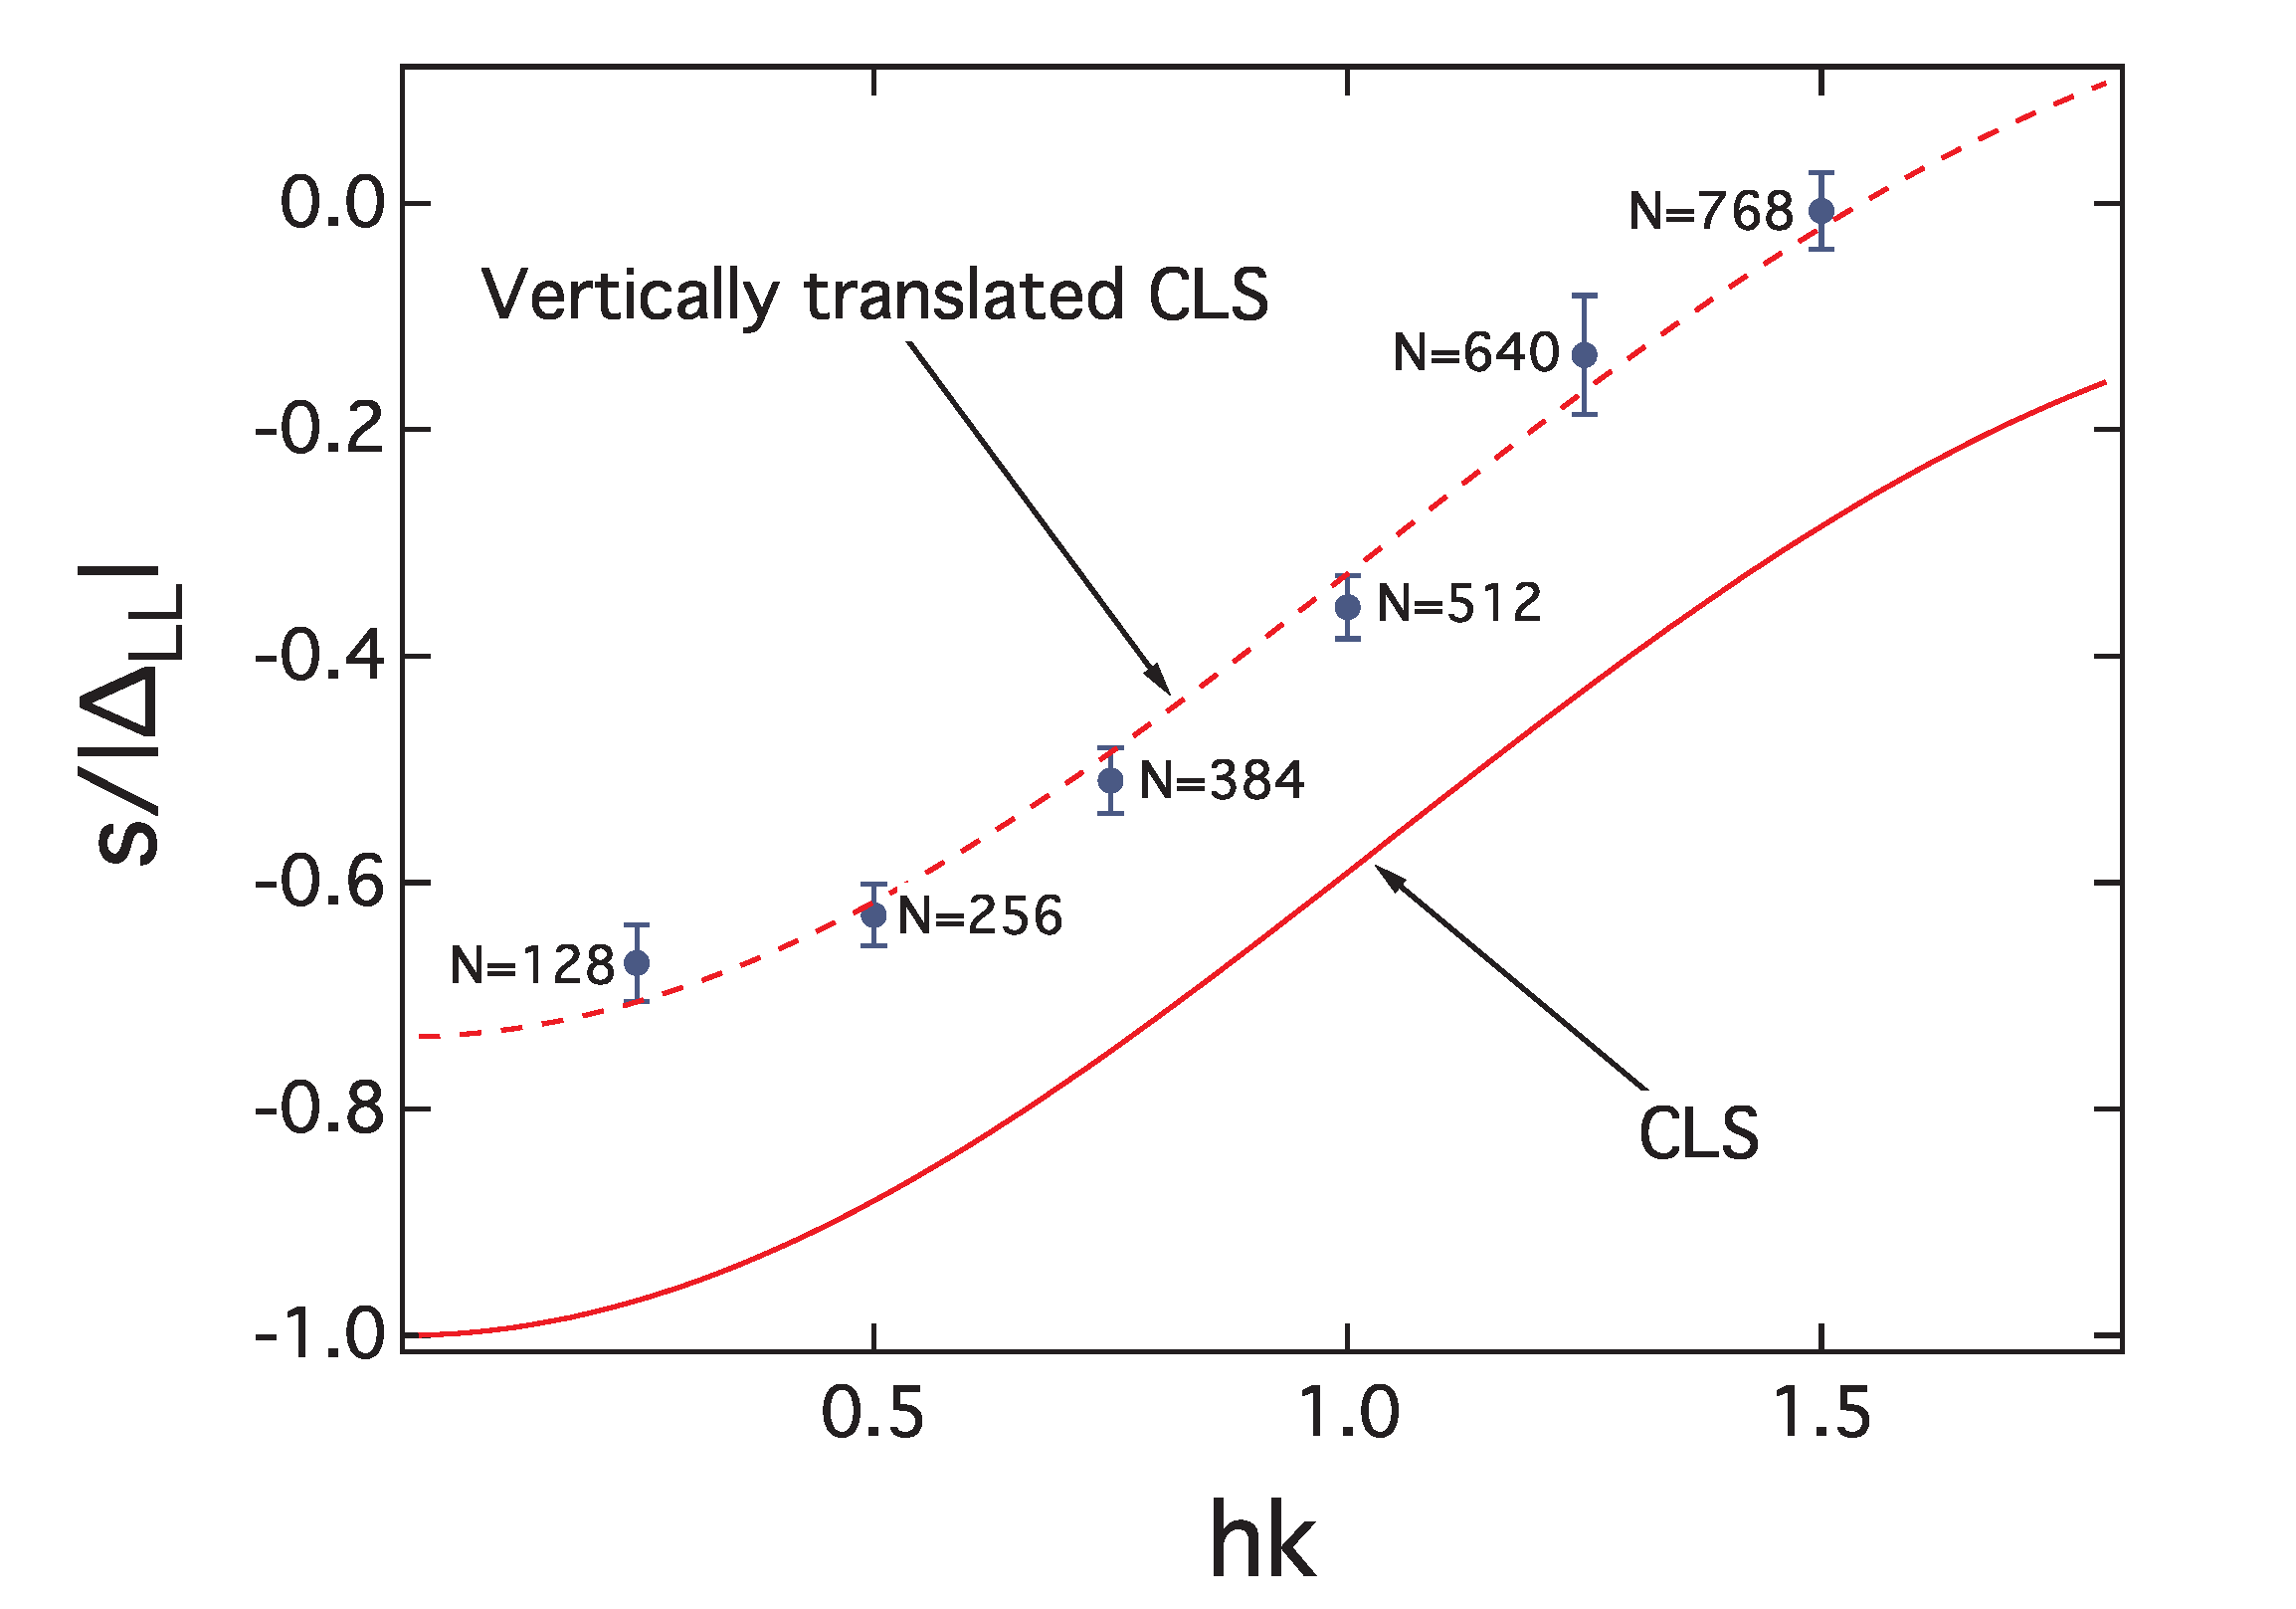
\includegraphics[width=\textwidth]{CLS.pdf}
\end{center}
\caption{The shift of the absorption line $s$ versus the thickness $h$ in a dense gas of moving atoms. $\Delta_{LL}$ is the standard LL shift.}
\label{CLS}
\end{figure}

FIG.~\eq{CLS} shows similar oscillations of the numerical and theoretical CLS. The dashed line is the vertically translated version of the theory. Note that no matter in the experiments ~cite{PhysRevLett.108.173601}, stationary-atom simulations ~cite{PhysRevLett.112.113603} or moving-atom simulations, there is always an additive constant to fit the data points.  The maximum atom number we have tested is $N=768$, for our simulation is restricted by the computing power. This result provides anther proof of the validity of our simulation program.

Similarly to stationary atoms, when the disk is very thin ($hk=0.25$ and $N=128$ in this case), the numerical result deviates from the curve because two dimensional behavior becomes important at this thickness.

\subsection{Broadening of the Dicke-narrowed lineshape in a Dense Gas}

By varying the density of the gas, we found new signs of coorporative effects in the absorption spectra.

\begin{figure}[h!]
\begin{center}
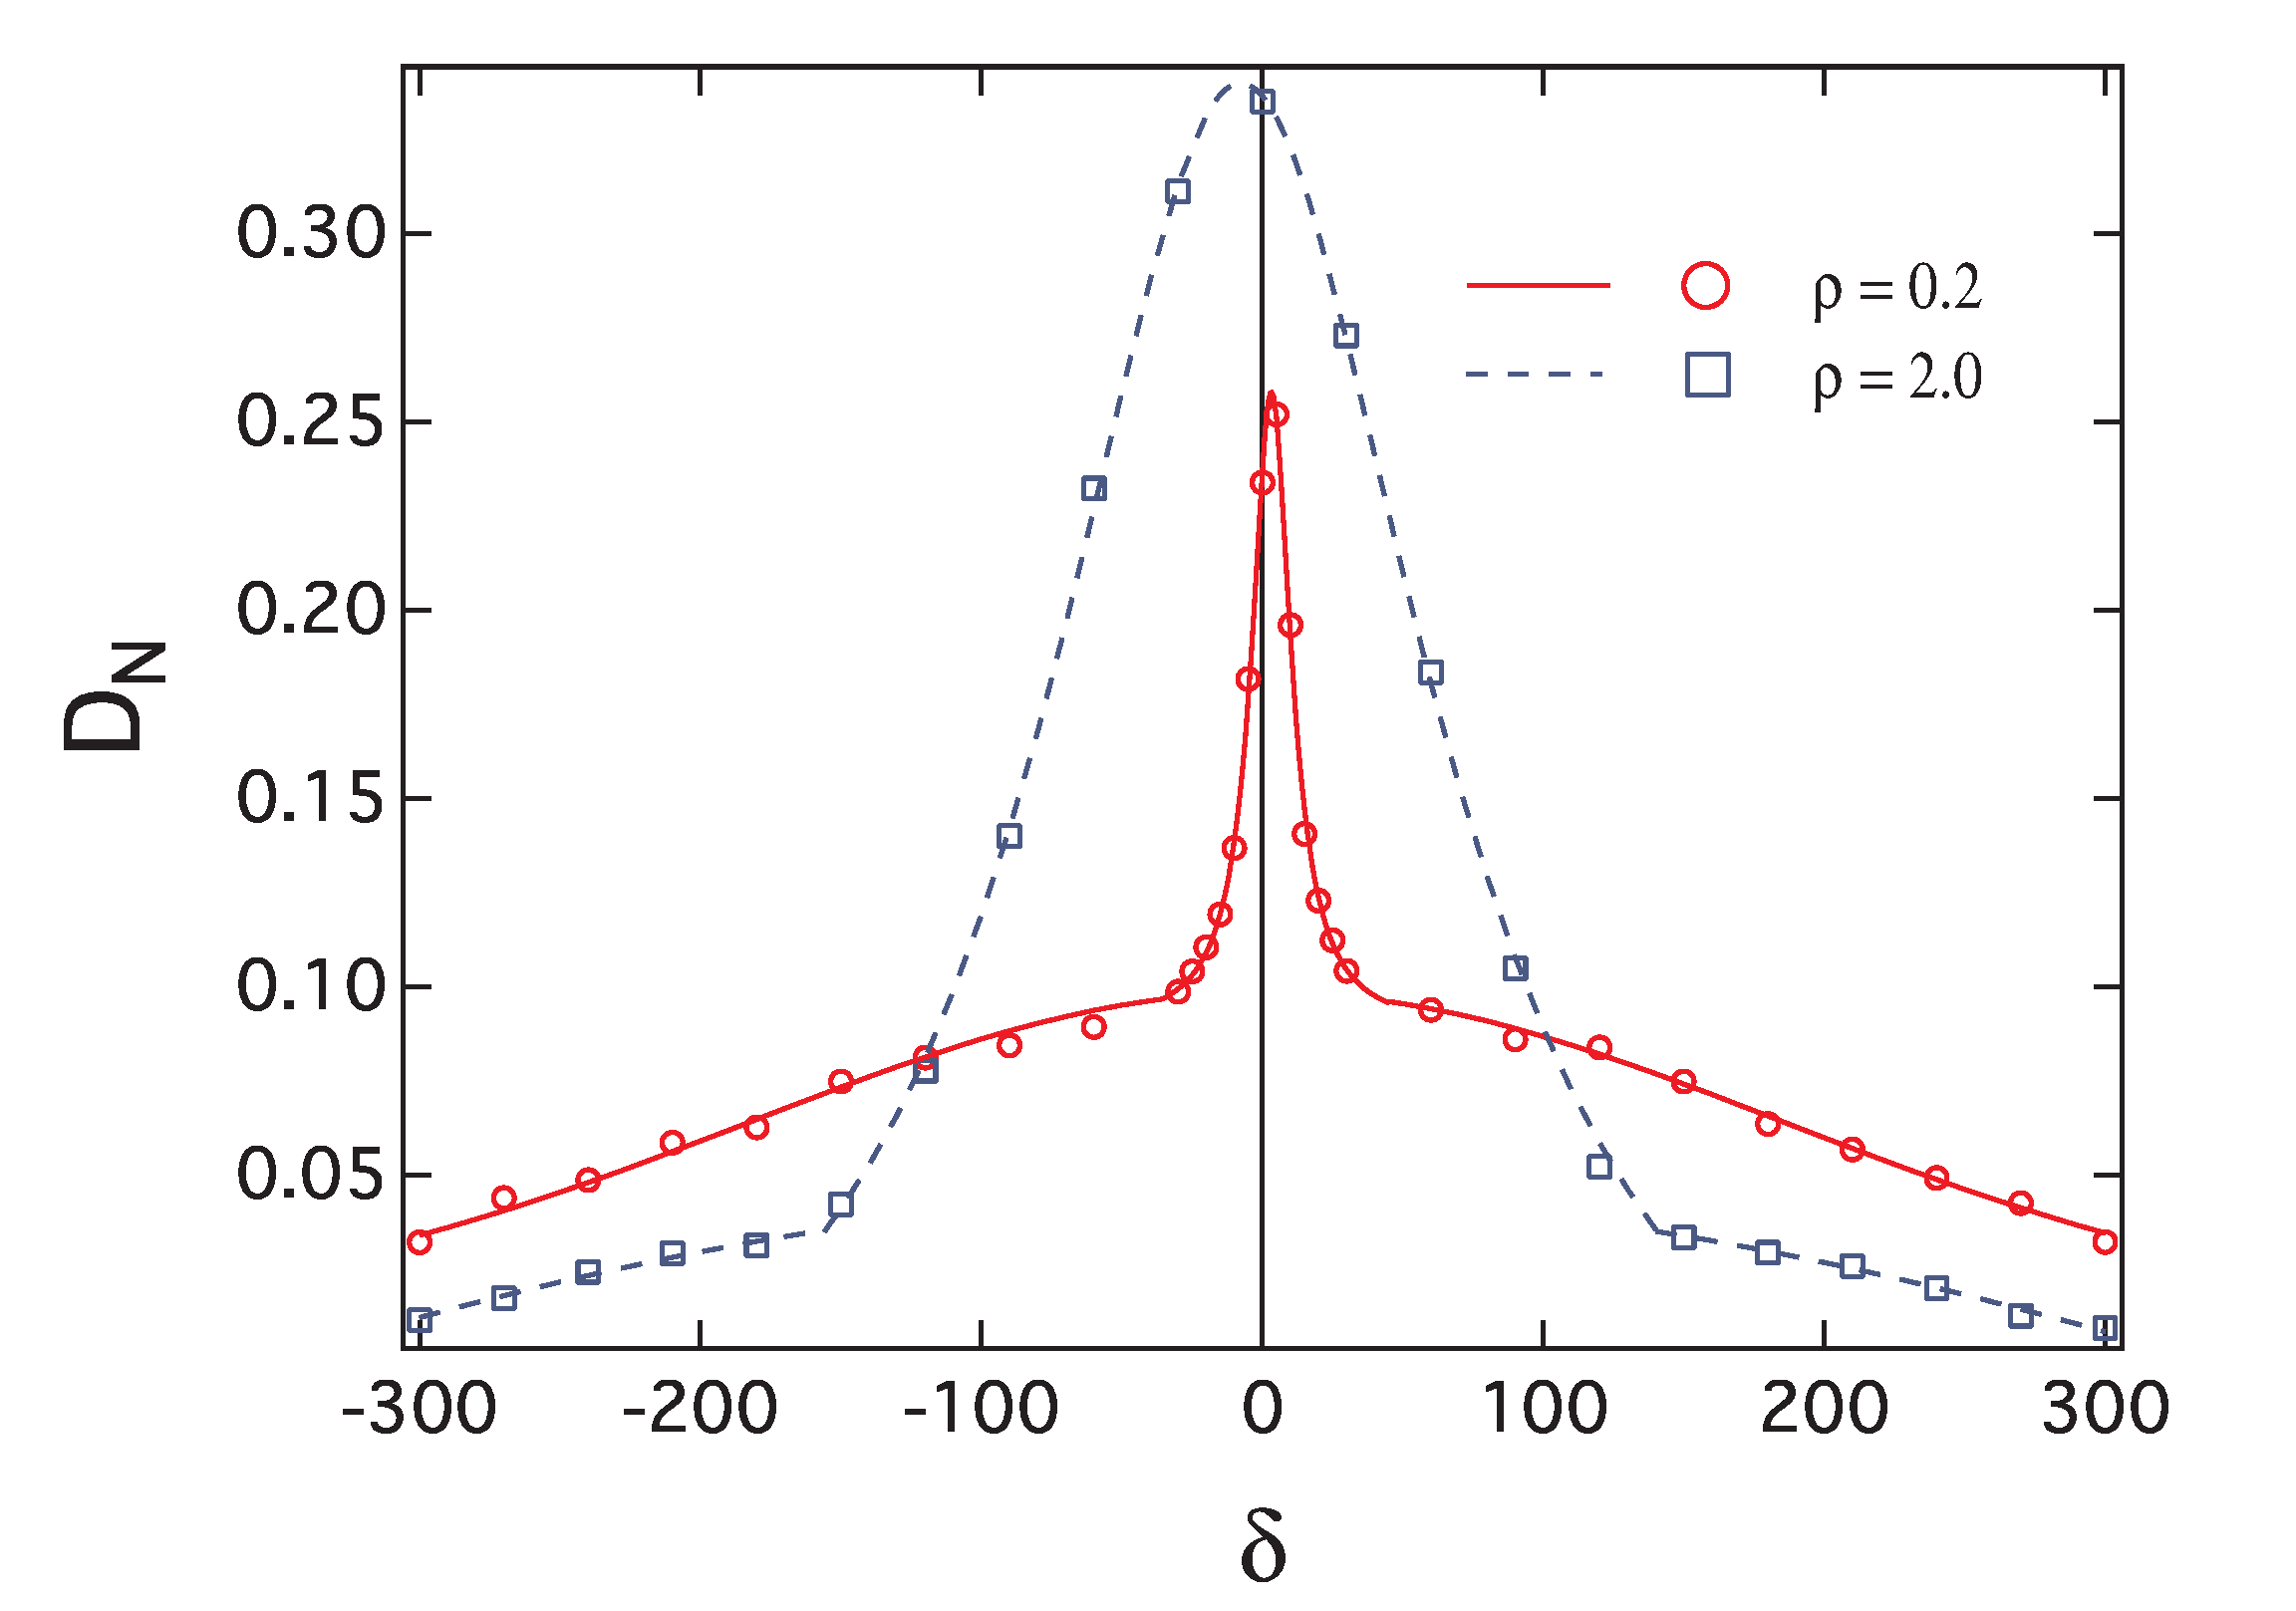
\includegraphics[width=\textwidth]{DICKE.pdf}
\end{center}
\caption{Optical thickness $D_N$ versus $\delta$ in two samples with different densities but the same number of atoms $N=256$. The thickness of the disk $h=5$ (red) and $0.5$ (blue) respectively. In both cases, the rms velocity of atoms $u=5$ and $R=\sqrt{256/\pi}$. The radius of an atom is $r_a=0.01$, so atom-atom collisions are very rare.}
\label{DICKE}
\end{figure}

As shown in FIG.~\eq{DICKE},  in a dilute gas ($\rho k^3=0.2$), based on a Gaussian profile from inhomogenous broadening, a very sharp Lorentzian peak arises near resonance. This is a typical phenomenon of Dicke narrowing. Note that in Sec. II, we also have a narrowing effect on the lineshape from collisions, nevertheless, what we observed there is more like a continuous transition from Gaussian to Lorentzian, not an abrupt Lorentzian peak right over a Gaussian base. So we may conclude here that in a classical gas, the typical appearance of a Dicke narrowed spectrum does not merely result from collision. In order to produce such a lineshape, dipole-dipole interactions (i.e. cooperative effects) must be present.

In the high density regime ($\rho k^3=2$) , the spectrum is still composed of two parts: Gaussian in the side wings and Lorentzian in the center. However, the central peak, as a signature of Dicke narrowing, is remarkably broadened, although the collision rate is much higher.

\begin{figure}[h!]
\begin{center}
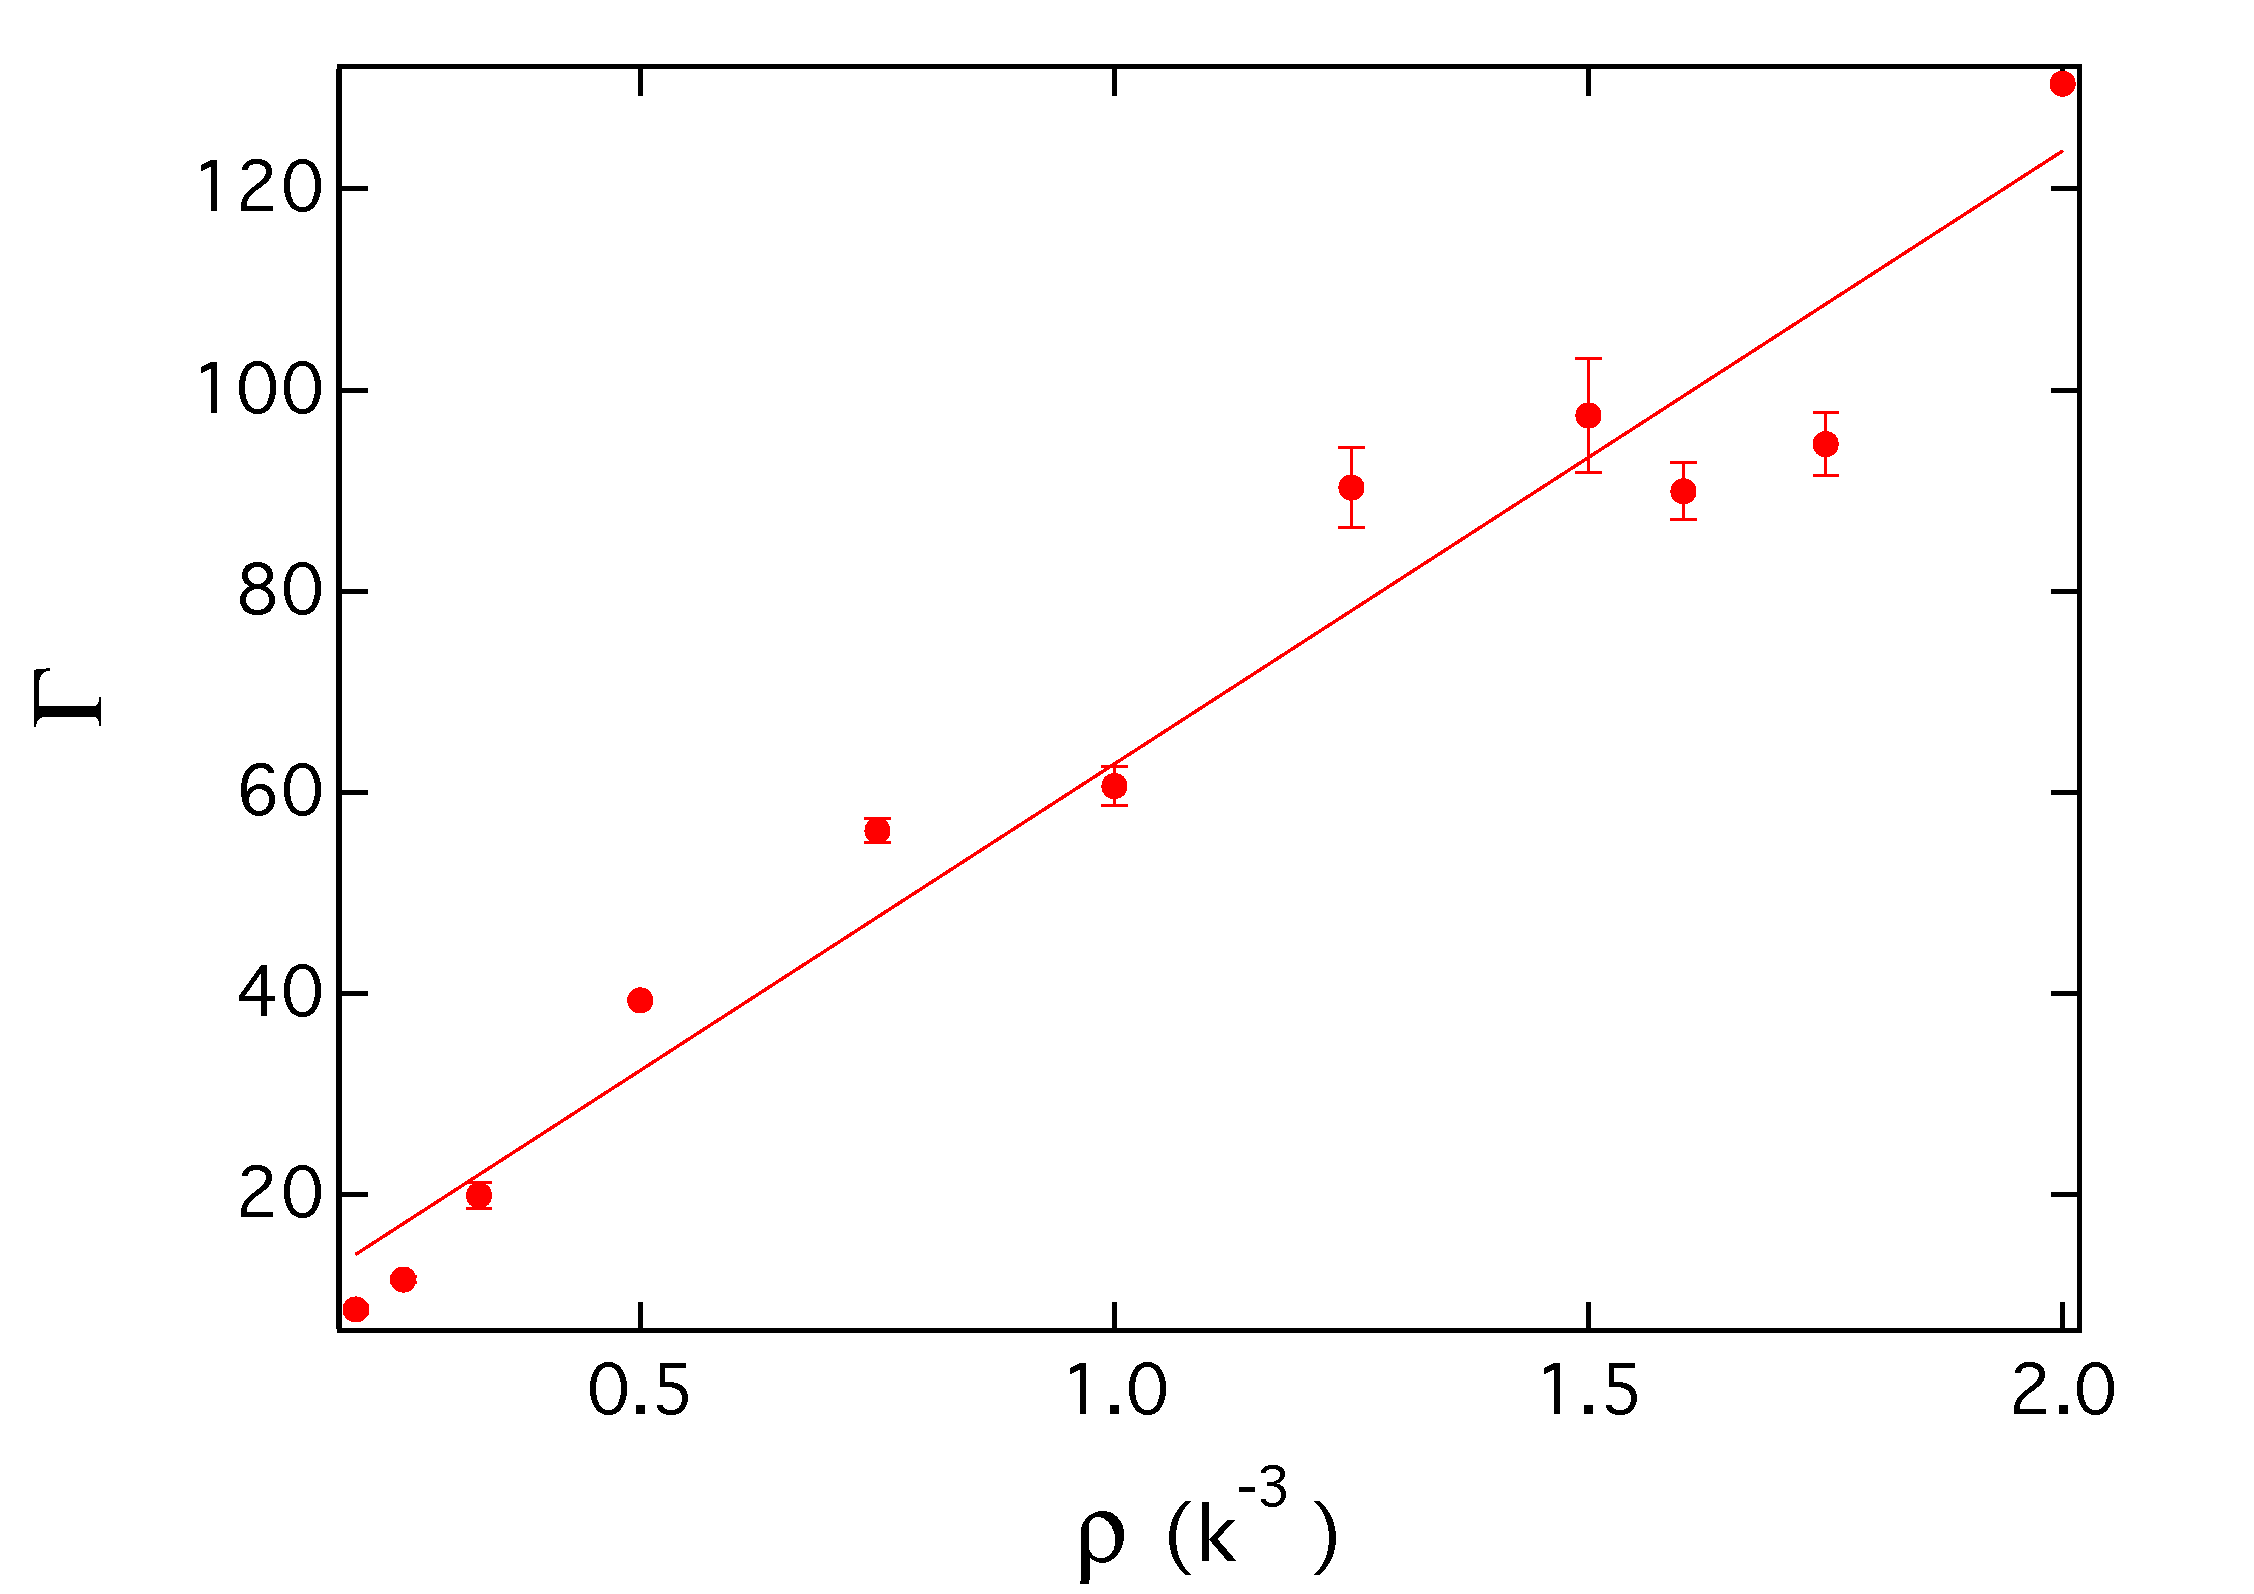
\includegraphics[width=\textwidth]{FWHM.pdf}
\end{center}
\caption{FWHM of the Lorentzian peak vs. density for same number of atoms $N=256$. The density is changed by varying the thickness of the disk.}
\label{FWHM}
\end{figure}

Recall the results we obtained in Sec. II, without dipole-dipole interactions, a higher frequency of either atom-wall collisions or atom-atom collisions would always narrow the lineshape. Conversely, when dipole-dipole interactions kick in, as shown in FIG.~\eq{FWHM}, the width of the Lorentzian peak in the spectrum keeps increasing as the density goes up. 

This broadening shows difference from a conventional Dicke narrowing phenomenon. It can by no means be classified as a collisional broadening, because the rigid sphere model is used all through our simulations thus the internal state of the atom is not considered at all. Since all of our work is done classically,  comparing to the results in Sec. II, we conclude that this broadening is a cooperative effect because of the light re-scattering processes between atoms.
